\documentclass[UTF8,fontset=none,12pt]{ctexart}

\setCJKmainfont{Songti SC}
\setCJKsansfont{PingFang SC}
\setCJKmonofont{Songti SC}

\usepackage[a4paper,margin=2.35cm]{geometry}
\usepackage{amsmath,amssymb,amsthm,mathtools,bm}
\usepackage{graphicx}
\usepackage{float}
\usepackage{booktabs}
\usepackage{array}
\usepackage{enumitem}
\usepackage[hidelinks]{hyperref}

\newcommand{\epsmach}{\varepsilon_{\mathrm{machine}}}
\theoremstyle{definition}
\newtheorem{theorem}{定理}
\renewcommand{\thetheorem}{20.\arabic{theorem}}

\title{数值线性代数\quad 第 20 讲：高斯消去法}
\author{Lloyd N. Trefethen、David Bau III\quad 中文阅读版}
\date{}

\begin{document}
\maketitle
\pagestyle{plain}

高斯消去法对读者来说想必并不陌生。它是手算线性方程组最简单的方法，也是计算机求解线性方程组的标准方法。本讲先介绍不带主元选取的纯粹高斯消去法；下一讲再加入对稳定性至关重要的行选主元操作。

\section*{LU 分解}

高斯消去法通过在左侧施加简单的线性变换，把一个完整的线性方程组变成上三角方程组。这一点与用 Householder 三角化计算 QR 分解相似；区别在于，高斯消去法使用的变换不是酉变换。

设 $A\in\mathbb{C}^{m\times m}$ 为方阵。（该算法也可用于矩形矩阵，但实践中很少这样做，所以本讲只讨论方阵。）我们的目标是通过在对角线下方逐列引入零元，把 $A$ 化为一个 $m\times m$ 上三角矩阵 $U$；先处理第 1 列，再处理第 2 列，依此类推，这与 Householder 三角化完全类似。具体做法是从后续各行中减去当前行的适当倍数。这个“消去”过程等价于在左侧依次乘以下三角矩阵 $L_k$：

\begin{equation}
    \underbrace{L_{m-1}\cdots L_2L_1}_{L^{-1}}A=U.
\tag{20.1}
\end{equation}

令

$$
L=L_1^{-1}L_2^{-1}\cdots L_{m-1}^{-1},
$$

就得到 $A=LU$，即

\begin{equation}
    A=LU,
\tag{20.2}
\end{equation}

其中 $U$ 是上三角矩阵，$L$ 是下三角矩阵。事实上，$L$ 是单位下三角矩阵，也就是说它的所有对角元都等于 1。

例如，从一个 $4\times4$ 矩阵开始时，算法分三步进行（可与式 (10.1) 对照）：

\begin{equation*}
\begin{bmatrix}
\times&\times&\times&\times\\
\times&\times&\times&\times\\
\times&\times&\times&\times\\
\times&\times&\times&\times
\end{bmatrix}
\xrightarrow{L_1}
\begin{bmatrix}
\times&\times&\times&\times\\
0&\times&\times&\times\\
0&\times&\times&\times\\
0&\times&\times&\times
\end{bmatrix}
\xrightarrow{L_2}
\begin{bmatrix}
\times&\times&\times&\times\\
0&\times&\times&\times\\
0&0&\times&\times\\
0&0&\times&\times
\end{bmatrix}
\xrightarrow{L_3}
\begin{bmatrix}
\times&\times&\times&\times\\
0&\times&\times&\times\\
0&0&\times&\times\\
0&0&0&\times
\end{bmatrix}.
\end{equation*}

（和第 10 讲一样，加粗表示刚刚操作过的条目，空白条目表示零。）第 $k$ 个变换 $L_k$ 通过从第 $k+1,\ldots,m$ 行中减去第 $k$ 行的适当倍数，在第 $k$ 列对角线下方引入零。由于第 $k$ 行前 $k-1$ 个条目已经是零，这一操作不会破坏之前引入的零。

因此，高斯消去法扩充了我们对矩阵分解算法的分类：

\begin{align*}
\text{Gram--Schmidt:}\quad &A=QR,\quad \text{通过三角正交化；}\\
\text{Householder:}\quad &A=QR,\quad \text{通过正交三角化；}\\
\text{高斯消去法:}\quad &A=LU,\quad \text{通过三角三角化}.
\end{align*}

\section*{例子}

讨论细节之前，先看一个数值例子。设

\begin{equation}
A=
\begin{bmatrix}
2&1&1&0\\
4&3&3&1\\
8&7&9&5\\
6&7&9&8
\end{bmatrix}.
\tag{20.3}
\end{equation}

$A$ 中的数字并非随机选择；它们被特意选取为能产生简单的 LU 分解。高斯消去的第一步为

\begin{equation*}
L_1A=
\begin{bmatrix}
1&0&0&0\\
-2&1&0&0\\
-4&0&1&0\\
-3&0&0&1
\end{bmatrix}
\begin{bmatrix}
2&1&1&0\\
4&3&3&1\\
8&7&9&5\\
6&7&9&8
\end{bmatrix}
=
\begin{bmatrix}
2&1&1&0\\
0&1&1&1\\
0&3&5&5\\
0&4&6&8
\end{bmatrix}.
\end{equation*}

也就是说，我们从第二行减去第一行的 2 倍，从第三行减去第一行的 4 倍，从第四行减去第一行的 3 倍。第二步为

\begin{equation*}
L_2L_1A=
\begin{bmatrix}
1&0&0&0\\
0&1&0&0\\
0&-3&1&0\\
0&-4&0&1
\end{bmatrix}
\begin{bmatrix}
2&1&1&0\\
0&1&1&1\\
0&3&5&5\\
0&4&6&8
\end{bmatrix}
=
\begin{bmatrix}
2&1&1&0\\
0&1&1&1\\
0&0&2&2\\
0&0&2&4
\end{bmatrix}.
\end{equation*}

这一次，我们从第三行减去第二行的 3 倍，从第四行减去第二行的 4 倍。最后，在第三步中从第四行减去第三行：

\begin{equation*}
L_3L_2L_1A=
\begin{bmatrix}
1&0&0&0\\
0&1&0&0\\
0&0&1&0\\
0&0&-1&1
\end{bmatrix}
\begin{bmatrix}
2&1&1&0\\
0&1&1&1\\
0&0&2&2\\
0&0&2&4
\end{bmatrix}
=
\begin{bmatrix}
2&1&1&0\\
0&1&1&1\\
0&0&2&2\\
0&0&0&2
\end{bmatrix}
=U.
\end{equation*}

现在，为了写出完整的分解 $A=LU$，需要计算

$$
L=L_1^{-1}L_2^{-1}L_3^{-1}.
$$

出人意料的是，这一步非常简单。$L_1$ 的逆矩阵就是把其对角线下方的每个条目变号：

\begin{equation}
\begin{bmatrix}
1&0&0&0\\
-2&1&0&0\\
-4&0&1&0\\
-3&0&0&1
\end{bmatrix}^{-1}
=
\begin{bmatrix}
1&0&0&0\\
2&1&0&0\\
4&0&1&0\\
3&0&0&1
\end{bmatrix}.
\tag{20.4}
\end{equation}

同样，$L_2$ 和 $L_3$ 的逆矩阵也只需将其次对角线条目变号。最后，$L_1^{-1}L_2^{-1}L_3^{-1}$ 正好是一个单位下三角矩阵：把 $L_1^{-1}$、$L_2^{-1}$ 和 $L_3^{-1}$ 的非零次对角线条目放到适当的位置即可。因此

\begin{equation}
\begin{bmatrix}
2&1&1&0\\
4&3&3&1\\
8&7&9&5\\
6&7&9&8
\end{bmatrix}
=
\begin{bmatrix}
1&0&0&0\\
2&1&0&0\\
4&3&1&0\\
3&4&1&1
\end{bmatrix}
\begin{bmatrix}
2&1&1&0\\
0&1&1&1\\
0&0&2&2\\
0&0&0&2
\end{bmatrix}.
\tag{20.5}
\end{equation}

\section*{一般公式与两次“幸运”}

下面给出 $m\times m$ 矩阵的一般公式。设 $x_k$ 表示第 $k$ 步开始时矩阵的第 $k$ 列。那么变换 $L_k$ 必须满足

\begin{equation*}
x_k=
\begin{bmatrix}
x_{1k}\\
\vdots\\
x_{kk}\\
x_{k+1,k}\\
\vdots\\
x_{mk}
\end{bmatrix}
\xrightarrow{L_k}
L_kx_k=
\begin{bmatrix}
x_{1k}\\
\vdots\\
x_{kk}\\
0\\
\vdots\\
0
\end{bmatrix}.
\end{equation*}

为此，我们希望从第 $j$ 行减去第 $k$ 行的 $\ell_{jk}$ 倍，其中乘子为

\begin{equation}
\ell_{jk}=\frac{x_{jk}}{x_{kk}},
\qquad k<j\le m.
\tag{20.6}
\end{equation}

矩阵 $L_k$ 的形式为

\begin{equation*}
L_k=
\begin{bmatrix}
1&&&&\\
&\ddots&&&\\
&&1&&\\
&&-\ell_{k+1,k}&1&\\
&&\vdots&&\ddots\\
&&-\ell_{mk}&&1
\end{bmatrix},
\end{equation*}

其中非零的次对角线条目位于第 $k$ 列。这与 Householder 三角化中的式 (10.2) 相似。

在上面的数值例子中，我们看到了两次“幸运”：$L_k$ 可以通过将其次对角线条目变号来求逆（式 (20.4)），而 $L$ 可以通过把这些 $\ell_{jk}$ 放到适当位置来构造（式 (20.5)）。下面解释为什么会这样。定义

\begin{equation*}
\ell_k=
\begin{bmatrix}
0\\
\vdots\\
0\\
\ell_{k+1,k}\\
\vdots\\
\ell_{mk}
\end{bmatrix}.
\end{equation*}

于是

$$
L_k=I-\ell_ke_k^*,
$$

其中 $e_k$ 是第 $k$ 个分量为 1、其余分量为 0 的列向量。由于 $\ell_k$ 的稀疏结构，有 $e_k^*\ell_k=0$，因此

$$
(I-\ell_ke_k^*)(I+\ell_ke_k^*)
=I-\ell_ke_k^*\ell_ke_k^*
=I.
$$

换句话说，

$$
L_k^{-1}=I+\ell_ke_k^*,
$$

这正是式 (20.4) 的形式。

第二次“幸运”可以这样说明。考虑相邻两个因子的乘积。由 $\ell_{k+1}$ 的稀疏结构，有 $e_k^*\ell_{k+1}=0$，因此

\begin{equation*}
\begin{aligned}
L_k^{-1}L_{k+1}^{-1}
&=(I+\ell_ke_k^*)(I+\ell_{k+1}e_{k+1}^*)\\
&=I+\ell_ke_k^*+\ell_{k+1}e_{k+1}^*.
\end{aligned}
\end{equation*}

所以 $L_k^{-1}L_{k+1}^{-1}$ 只是一个单位下三角矩阵，其中包含 $L_k^{-1}$ 与 $L_{k+1}^{-1}$ 的条目，并且这些条目位于各自通常的下三角位置。把所有矩阵相乘形成 $L$ 时，整个对角线下方都具有同样的便利结构：

\begin{equation}
L=L_1^{-1}L_2^{-1}\cdots L_{m-1}^{-1}
=
\begin{bmatrix}
1&&&\\
\ell_{21}&1&&\\
\ell_{31}&\ell_{32}&1&\\
\vdots&\vdots&\ddots&\ddots\\
\ell_{m1}&\ell_{m2}&\cdots&\ell_{m,m-1}&1
\end{bmatrix}.
\tag{20.7}
\end{equation}

第 8 讲没有提到，导致式 (20.7) 的稀疏性考察，其实也出现在式 (8.10) 对改进 Gram–Schmidt 过程的解释中：那里是一系列右乘三角矩阵 $R_k$。

在实际高斯消去法中，从来不会显式形成并相乘矩阵 $L_k$。乘子 $\ell_{jk}$ 会直接计算并存储到 $L$ 中，然后隐式应用变换 $L_k$。

\subsection*{算法 20.1\quad 不带主元的高斯消去法}

\begin{verbatim}
U = A, L = I
for k = 1 to m - 1
    for j = k + 1 to m
        l_jk = u_jk/u_kk
        u_j,k:m = u_j,k:m - l_jk u_k,k:m
\end{verbatim}

（实际上不需要三个矩阵 $A,L,U$；为了节省计算机内存，$L$ 和 $U$ 可以写入与 $A$ 相同的数组中。）习题 20.4 给出了高斯消去法的另一种“外积”形式：它只包含一个显式循环，而不是两个。

\section*{运算量}

和往常一样，可以从几何上推导这个算法的渐近运算量。主要工作是内层循环中的向量操作

$$
u_{j,k:m}=u_{j,k:m}-\ell_{jk}u_{k,k:m},
$$

它执行一次标量–向量乘法和一次向量减法。若 $l=m-k+1$ 表示正在处理的行向量长度，则每个条目的浮点运算次数为 2，因此这一行需要 $2l$ 次浮点运算。

对每个 $k$，内层循环要处理第 $k+1,\ldots,m$ 行。相应的工作量是下图立体的一层：

\begin{figure}[H]
    \centering
    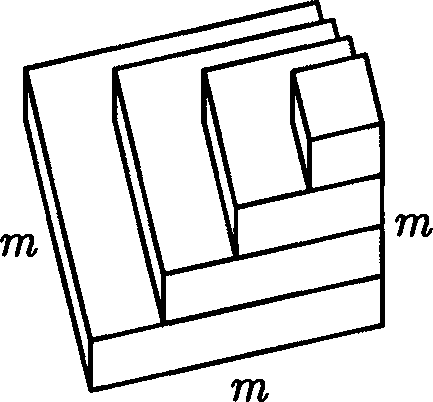
\includegraphics[width=0.48\textwidth]{../assets/figure-20-1.png}
    \caption{表示高斯消去法运算量的立体图。}
\end{figure}

这与第 10 讲中用来表示 Householder 三角化工作量的图相同（这里假设 $m=n$）。不过在那里，每个单位立方体代表 4 次浮点运算，而不是 2 次。和之前一样，当 $m\to\infty$ 时，这个立体趋近于一个体积为 $\frac13m^3$ 的棱锥。每单位体积包含 2 次浮点运算，所以

\begin{equation}
\text{高斯消去法的运算量}\ \sim\ \frac23m^3\ \text{次浮点运算}.
\tag{20.8}
\end{equation}

\section*{用 LU 分解求解 $Ax=b$}

如果 $A$ 已分解为 $L$ 和 $U$，方程组 $Ax=b$ 就化为

$$
LUx=b.
$$

因此可以分两步求解两个三角系统：先求未知向量 $y$，解 $Ly=b$（前代）；再求未知向量 $x$，解 $Ux=y$（回代）。第一步，即分解阶段，需要约 $\frac23m^3$ 次浮点运算；第二、三步各需要约 $m^2$ 次浮点运算。因此总运算量约为 $\frac23m^3$ 次浮点运算，是用 Householder 三角化（算法 16.1）求解时约 $\frac43m^3$ 次浮点运算（式 (10.9)）的一半。

为什么求解方阵方程组时通常使用高斯消去法，而不是 QR 分解？运算量约为一半当然是原因之一。不过，同样重要的可能还有历史因素：消去法已经存在了几个世纪，而矩阵的 QR 分解直到计算机发明之后才出现。若要取代高斯消去法成为首选方法，QR 分解必须具有非常有说服力的优势。

\section*{不带主元高斯消去法的不稳定性}

遗憾的是，到目前为止介绍的高斯消去法不能用于求解一般线性方程组，因为它不是后向稳定的。这种不稳定性还关联着一个更明显的困难：对某些矩阵，高斯消去法会因为尝试除以零而完全失败。

例如，考虑

$$
A=\begin{bmatrix}0&1\\1&1\end{bmatrix}.
$$

这个矩阵满秩且良态，其 2-范数条件数为 $\kappa_2(A)=\frac{3+\sqrt5}{2}\approx2.618$。

然而，高斯消去法在第一步就会失败。

对同一个矩阵做一个微小扰动，可以看出更一般的问题。设

\begin{equation}
A=
\begin{bmatrix}
10^{-20}&1\\
1&1
\end{bmatrix}.
\tag{20.9}
\end{equation}

这一次过程不会失败。相反，需要从第二行中减去第一行的 $10^{20}$ 倍，得到以下因子：

$$
L=\begin{bmatrix}1&0\\10^{20}&1\end{bmatrix},
\qquad
U=\begin{bmatrix}10^{-20}&1\\0&1-10^{20}\end{bmatrix}.
$$

现在假设计算在浮点算术中进行，且 $\epsmach\approx10^{-16}$。数 $1-10^{20}$ 无法被精确表示，会被舍入到最近的浮点数。为简单起见，假设它恰好被舍入为 $-10^{20}$。于是算法产生的浮点矩阵为

$$
\widetilde{L}=\begin{bmatrix}1&0\\10^{20}&1\end{bmatrix},
\qquad
\widetilde{U}=\begin{bmatrix}10^{-20}&1\\0&-10^{20}\end{bmatrix}.
$$

一开始，这种程度的舍入似乎还可以接受。毕竟，相对于 $\|\widetilde U\|$ 而言，矩阵 $\widetilde U$ 与正确的 $U$ 很接近。然而，当我们计算乘积 $\widetilde L\widetilde U$ 时，问题就暴露出来了：

$$
\widetilde L\widetilde U=
\begin{bmatrix}
10^{-20}&1\\
1&0
\end{bmatrix}.
$$

这个矩阵与 $A$ 完全不接近，因为 $(2,2)$ 位置的 1 被替换成了 0。如果现在求解系统 $\widetilde L\widetilde U\widetilde x=b$，结果将与 $Ax=b$ 的解完全不同。例如取 $b=(1,0)^T$，得到

$$
\widetilde x=(0,1)^T,
$$

而正确解为 $x\approx(-1,1)^T$。

仔细考察这个例子，可以得到如下结论。高斯消去法稳定地计算出了 LU 分解：$\widetilde L$ 和 $\widetilde U$ 是某个接近 $A$ 的矩阵的精确因子（事实上，这个矩阵就是 $A$ 本身附近的矩阵）。然而，它并没有稳定地求解 $Ax=b$。原因在于：LU 分解虽然是稳定的，却不是后向稳定的。一般而言，如果一个算法的某一步是稳定但不是后向稳定的子问题求解算法，那么整个计算的稳定性就可能受到威胁。

事实上，对于一般的 $m\times m$ 矩阵 $A$，情况还要更糟。不带主元的高斯消去法作为 LU 分解的一般算法，既不是后向稳定的，也不是稳定的。此外，它生成的三角矩阵的条件数可能任意大于 $A$ 的条件数，从而在求解 $Ax=b$ 的前代和回代阶段引入额外的不稳定来源。

\section*{习题}

\begin{enumerate}[label=\textbf{20.\arabic*}]
    \item 设 $A\in\mathbb{C}^{m\times m}$ 非奇异。证明：$A$ 存在 LU 分解，当且仅当对每个 $1\le k\le m$，其左上角 $k\times k$ 子块 $A_{1:k,1:k}$ 非奇异。（提示：高斯消去的行操作不改变 $\det(A_{1:k,1:k})$。）证明这个 LU 分解是唯一的。

    \item 假设 $A\in\mathbb{C}^{m\times m}$ 满足习题 20.1 的条件，并且带宽为 $2p+1$，即当 $|i-j|>p$ 时有 $a_{ij}=0$。关于 $A$ 的因子 $L$ 和 $U$ 的稀疏结构，你能得到什么结论？

    \item 设一个 $m\times m$ 矩阵 $A$ 写成分块形式
    \[
    A=\begin{bmatrix}A_{11}&A_{12}\\A_{21}&A_{22}\end{bmatrix},
    \]
    其中 $A_{11}$ 是 $n\times n$，$A_{22}$ 是 $(m-n)\times(m-n)$。假设 $A$ 满足习题 20.1 的条件。

    \begin{enumerate}[label=(\alph*)]
        \item 验证公式
        \[
        \begin{bmatrix}
        I&0\\
        -A_{21}A_{11}^{-1}&I
        \end{bmatrix}
        \begin{bmatrix}
        A_{11}&A_{12}\\
        A_{21}&A_{22}
        \end{bmatrix}
        =
        \begin{bmatrix}
        A_{11}&A_{12}\\
        0&A_{22}-A_{21}A_{11}^{-1}A_{12}
        \end{bmatrix},
        \]
        这相当于“消去”分块 $A_{21}$。矩阵
        $A_{22}-A_{21}A_{11}^{-1}A_{12}$ 称为 $A$ 中 $A_{11}$ 的 Schur 补。

        \item 假设通过 $n$ 步高斯消去逐行消去 $A_{21}$。证明所得结果右下角的 $(m-n)\times(m-n)$ 分块仍然是
        $A_{22}-A_{21}A_{11}^{-1}A_{12}$。
    \end{enumerate}

    \item 和本书中的大多数算法一样，高斯消去法包含三重嵌套循环。在算法 20.1 中，有两个显式的 for 循环，第三个循环则隐含在向量 $u_{j,k:m}$ 和 $u_{k,k:m}$ 中。将该算法改写为只用一个按 $k$ 索引的显式 for 循环。在这个循环内部，每一步都通过某个秩一外积更新 $U$。如果想优化计算机性能，这种高斯消去的“外积”形式可能比算法 20.1 更适合作为起点。

    \item 我们已经看到，高斯消去得到 $A=LU$，其中 $L$ 的对角线为 1，而 $U$ 不一定如此。若按以下方式改变这个过程，请在高层次上描述所得的分解：
    \begin{enumerate}[label=(\alph*)]
        \item 从左到右按列消去，而不是从上到下按行消去，使 $A$ 变成下三角矩阵。
        \item 先用对角矩阵 $D$ 对 $A$ 的列做缩放，再进行高斯消去。在这种重新缩放下，方程组 $Ax=b$ 变成什么形式？由 $D$ 重新缩放的是方程还是未知量？
        \item 继续进行高斯消去：在把 $A$（假设非奇异）化为上三角矩阵之后，再进行额外的列操作，使这个上三角矩阵变成对角矩阵。
    \end{enumerate}
\end{enumerate}

\end{document}
